\documentclass[12pt,fleqn,x11names,table]{report}                                                  
\usepackage[text={15cm,25cm},centering,headsep=20pt,top=0.8in, bottom = 0.8in,letterpaper,showframe=false]{geometry}
%--------------------------------------------------------------------------
% Paquetes y estilo del libro. http://www.tec-digital.itcr.ac.cr/revistamatematica/
% Versi�n Juio-2014
%--------------------------------------------------------------------------
% Paquetes 
\usepackage[spanish,es-tabla]{babel}
\usepackage[latin1]{inputenc}                   % Entrada de acentos
\usepackage[T1]{fontenc}
\usepackage[autostyle, spanish = mexican]{csquotes}% manejo de comillas: " "
\MakeOuterQuote{"}
\usepackage{pslatex}                              % Fuentes finas postscript
%\usepackage[sc]{mathpazo}                         % Fuentes mathpazo
\usepackage{helvet}
\linespread{1.05}                                  % Fuente Palatino necesita espaciado
\usepackage[full]{textcomp}                        % Caracteres especiales como ' (recto)
\usepackage{xcolor}                                % Color: X11names (en el documentclass)
% COLORES personales---------------------------------------------------
    \definecolor{colortitulo}{RGB}{11,17,79} % 
    \definecolor{colordominante}{RGB}{11,17,79}
    \definecolor{colordominanteA}{RGB}{243,102,25}
    \definecolor{colordominanteF}{RGB}{219,68,14}
    \definecolor{colordominanteD}{RGB}{74,0,148}
   
    \definecolor{wcolornotas}{RGB}{74,0,148}%{RGB}{51,145,147} % 
    \definecolor{mostaza}{RGB}{231,196,25}
    \definecolor{amarilloM}{RGB}{248,199,90}
    \definecolor{amarilloD}{RGB}{251,237,121}
    \definecolor{azulF}{rgb}{.0,.0,.3}
    \definecolor{grisD}{rgb}{.3,.3,.3}
    \definecolor{grisF}{rgb}{.6,.6,.6}
    \definecolor{grisamarillo}{RGB}{248,248,245} 
    \definecolor{miverde}{RGB}{44,162,67}
    \definecolor{verdep}{RGB}{166,206,58}
    \definecolor{verdeF}{RGB}{5,92,8}
    \colorlet{mygray}{black!20}
    \newcommand{\verde}{\color{miverde}}
    \newcommand{\colornotas}{\color{wcolornotas}}
% Fin COLORES personales-------------------------------------------------
\usepackage{psboxit}
\usepackage{pstricks}
\usepackage{xparse}

\usepackage{tikz,tkz-tab}% Cajas de Teoremas, ejemplos, etc.
%listings para c�digo en color en tcbcolor
\usetikzlibrary{matrix,arrows,
positioning,shadows,shadings,backgrounds,calc, shapes, tikzmark}%
\usepackage{tcolorbox, empheq} 
 % Librer�as tcolorbox
\tcbuselibrary{skins,breakable,listings,theorems} 

\usepackage{xargs}                                 % Comandos con opciones
\DeclareGraphicsExtensions{.pdf,.png,.jpg}
\usepackage{multicol}
% %\usepackage{epstopdf}% Conversi�n - Miktes 2.9 o inferior, TexLive 2009. o inferior
\usepackage[small,bf,labelsep=period]{caption}
\usepackage[breaklinks,colorlinks=true, pdfstartview=FitV, linkcolor=azulF, citecolor=azulF, urlcolor=azulF]{hyperref}
\usepackage{amsmath,amssymb,amsfonts,latexsym,cancel,stmaryrd}%
\usepackage[ruled,,vlined,lined,linesnumbered,algochapter]{algorithm2e}
\usepackage{framed}
\usepackage{titletoc}
\usepackage{calc}
\usepackage{longtable} 
\usepackage{colortbl} 
\usepackage{tabularx}
\usepackage{fancyvrb}
%\usepackage{minted}   %habilitar solo en Ubuntu (Linux)
\usepackage{array}
\usepackage{wasysym}
\usepackage{supertabular}
\definecolor{verbmentsbgcolor}{rgb}{0.9764, 0.9764, 0.9762}
\definecolor{verbmentscaptionbgcolor}{rgb}{0.1647, 0.4980, 1}
\usepackage{verbments}
\fvset{frame=bottomline,framerule=0.01cm}
\plset{language=java,texcl=true,style=vs,%
listingnamefont=\sffamily\bfseries\color{white},%
bgcolor=verbmentsbgcolor,captionfont=\sffamily\color{white},%
captionbgcolor=verbmentscaptionbgcolor, listingname=\textbf{Programa}}
%\usepackage{pagecolor}
\usepackage[textwidth=2cm]{todonotes} 
\usepackage{booktabs}
\usepackage{marginnote}
\usepackage[b]{esvect}
\usepackage{rotating}
%\usepackage{float}
\usepackage{floatrow}
\usepackage[shortlabels]{enumitem}
\usepackage{subfigure}
\usepackage{wrapfig}
\usepackage{floatflt}
 \usepackage{kantlipsum} %\kant[1-13]

\renewcommand{\thechapter}{\roman{chapter}}
\renewcommand{\thesection}{\arabic{chapter}.\arabic{section}}
%----------------------------------------------------------------------------------------
% Fuentes especiales
%----------------------------------------------------------------------------------------
% Comandos para fuentes especiales
\newcommandx*{\fnte}[4][1=pag,2=9,3=n]{{\color{azulF}\fontfamily{#1}\fontseries{b}
\fontsize{#2}{1}\fontshape{#3}\selectfont{#4}}}

\newcommandx*{\fntb}[4][1=pag,2=9,3=n]{{\color{azulF}\fontfamily{#1}\fontsize{#2}{1}\fontseries{b}\fontshape{#3}\selectfont{#4}}}

\newcommandx*{\fntg}[4][1=pag,2=9,3=n]{{\color{grisF}\fontfamily{#1}\fontsize{#2}{1}\fontshape{#3}\selectfont{#4}}}

\newcommand{\fhv}[2]{{\fontfamily{pag}\fontsize{#1}{1}\selectfont{#2}}}

\newcommand{\fhvb}[2]{{\fontfamily{pag}\fontseries{b}\fontsize{#1}{1}\selectfont{#2}}}

% fontfamily %n = normal, it =italics
\newcommandx*{\fntl}[4][1=pag,2=10,3=n]{{\colornotas\fontfamily{#1}\fontsize{#2}{1}\fontseries{b}\fontshape{#3}\selectfont{#4}}}

\newcommandx*{\tfntl}[4][1=pag,2=10,3=n]{{\color{azulF}\fontfamily{#1}\fontsize{#2}{1}\fontseries{b}\fontshape{#3}\selectfont{#4}}}

\newcommandx*{\fnt}[4][1=pag,2=9,3=n]{{\colornotas\fontfamily{#1}\fontsize{#2}{1}\fontshape{#3}\selectfont{#4}}}

\newcommandx*{\colrfnt}[4][1=pag,2=9,3=n]{{\red\fontfamily{#1}\fontsize{#2}{1}\fontshape{#3}\selectfont{#4}}}

\newcommandx*{\nfnt}[4][1=pag,2=9,3=n]{{\fontfamily{#1}\fontsize{#2}{1}\fontshape{#3}\selectfont{#4}}}

\newcommand{\wfont}[2]{{\fontfamily{#1}\selectfont{#2}}}
\newcommand{\fptm}[1]{{\fontfamily{ptm}\selectfont{#1}}}

\newcommandx*{\cfnte}[4][1=pag,2=9,3=n]{{\wcelestetxt\fontfamily{#1}\fontsize{#2}{1}\fontshape{#3}\selectfont{#4}}}
% Fin fuentes----------------------------------------------------------

%----------------------------------------------------------------------------------------
% Cabeceras
%----------------------------------------------------------------------------------------
% Elimina el encabezado de las p�ginas impares vac�as al final de los cap�tulos
\makeatletter
\renewcommand{\cleardoublepage}{
\clearpage\ifodd\c@page\else
\hbox{}
\vspace*{\fill}
\thispagestyle{empty}
\newpage
\fi}
%\makeatother

\usepackage{fancyhdr}
% N�meros de p�gina en rect�ngulos y cap�tulo. Necesitamos posicionar los nodos
\usepackage[absolute]{textpos}
    \setlength{\TPHorizModule}{10mm}% 1 generic horizontal unit is equivalent to 10mm
    \setlength{\TPVertModule}{10mm}% 1 generic vertical unit is equivalent to 10mm
    \textblockorigin{0mm}{0mm}% top left corner set as origin

%\makeatletter
% Redefinir \chaptermark sin "cap�tulo" ni n�mero de cap�tulo, solo el texto.
\renewcommand{\chaptermark}[1]{\markboth{\if@mainmatter\ ~~\fi#1}{}}
\makeatother

%------------------------------------------------------------------------------
% Decoraci�n de cabeceras 
% Texto en secciones
\renewcommand{\sectionmark}[1]{\markright{\sffamily\normalsize\thesection\hspace{5pt}#1}{}} 
% Configuraci�n de fuentes para el n�mero de p�gina en el encabezado
\fancyhf{} 
% > OP 1: Todas las p�ginas con la secci�n a la izquierda
%   \fancyhead[LO,LE]{\rightmark} % L=Left, O=Odd y  E=Even pages
% > OP 2: Todas las p�ginas con la seci�n a la izquierda en un rect�ngulo (todo el header)
%   \usepackage{tikzpagenodes}
%   \fancyhead[LO,LE]{\rightmark
%   \begin{textblock}{1}(0,0)
%   \begin{tikzpicture}[remember picture,overlay]
%   \fill[grisamarillo] (current page.north west) 
%     rectangle
%   ([xshift=2pt,yshift=-3pt]current page.east|-current page header area.south east);
%   \end{tikzpicture}
%   \end{textblock}
%   }
% > OP 3: Todas las p�ginas con la seci�n a la izquierda en rect�ngulo bordes difusos
\usepackage{tikzpagenodes}
\usetikzlibrary{decorations.pathmorphing,calc,shadows.blur,shadings}
\pgfmathsetseed{1}

\pgfdeclaredecoration{irregular fractal line}{init}
{
  \state{init}[width=\pgfdecoratedinputsegmentremainingdistance]
  {
    \pgfpathlineto{\pgfpoint{random*\pgfdecoratedinputsegmentremainingdistance}{(random*\pgfdecorationsegmentamplitude-0.02)*\pgfdecoratedinputsegmentremainingdistance}}
    \pgfpathlineto{\pgfpoint{\pgfdecoratedinputsegmentremainingdistance}{0pt}}
  }
}

\tikzset{
   paper/.style={draw=black!10, blur shadow, shade=bilinear interpolation,
                 lower left=black!20, upper left=black!15, upper right=white, lower right=black!10},
   irregular border/.style={decoration={irregular fractal line, amplitude=0.2},
           decorate,
     },
   ragged border/.style={ decoration={random steps, segment length=7mm, amplitude=2mm},
           decorate,
   }
}
%L=Left, Odd Even - Decoraci�n en encabezado aqui entra el encabezado verde con titulo de ref http
\fancyhead[LO,LE]{}

% Fin decoraci�n cabeceras
\renewcommand{\headrulewidth}{0pt}   % Ancho de la l�nea bajo el encabezado
\addtolength{\headheight}{2.5pt}     % Aumente el espacio alrededor de la cabecera 
\renewcommand{\footrulewidth}{0pt}   % Elimina la l�nea en el pie de p�gina
% Estilo para  "pagestyle plain"
\fancypagestyle{plain}{\fancyhead{}\renewcommand{\headrulewidth}{0pt}} 



% N�meros de p�gina+chaptertitle en rect�ngulo en el borde
\fancyfoot[LE]{
\begin{textblock}{3}(21,5)
\begin{tikzpicture}[overlay]
\node[draw=colordominante,
rectangle,minimum width=2cm, minimum height=2cm,
anchor=west,
fill=colordominante,font=\fontsize{25}{1}\sffamily\bfseries,inner sep=2pt,outer sep=2pt] 
at (-1.5cm,0pt){\textcolor{gray!10}{\thepage}};
%cap
\node[right,line width=1pt,rectangle,
fill=grisamarillo,font=\fontsize{35}{1}\sffamily\bfseries,inner sep=20pt,outer sep=60pt,
rotate=-90] at (current page.south west){\textcolor{gray!30}{\leftmark}};  
\end{tikzpicture}
\end{textblock}
}

\fancyfoot[RO]{
\begin{textblock}{3}(18,5)
\begin{tikzpicture}[overlay]
\node[draw=colordominante,rectangle,minimum width=2cm, minimum height=2cm,
anchor=west,
fill=colordominante,font=\fontsize{25}{1}\sffamily\bfseries,inner sep=2pt,outer sep=2pt] 
at (-1.5cm,0pt){\textcolor{gray!10}{\thepage}};
% %cap
% \node[left,line width=1pt,rectangle,
% fill=grisamarillo,font=\fontsize{35}{1}\sffamily\bfseries,inner sep=20pt,outer sep=60pt,
% rotate=90]at (current page.south west){\textcolor{gray!30}{\leftmark}};    
\end{tikzpicture}
\end{textblock}
}
\setlength\headheight{14.5pt} % 
% Fin cabeceras 

%----------------------------------------------------------------------------------------
% Color en los m�rgenes
%----------------------------------------------------------------------------------------
% \pagecolor{grisamarillo}
% \usepackage{eso-pic}
% \pagecolor{grisamarillo}
% \AddToShipoutPictureBG{%
%  \AtTextLowerLeft{\color{grisamarillo}%
%   \rule[-\footskip]{\textwidth}{\dimexpr\textheight+\footskip}}}

% Fin color m�rgenes


%----------------------------------------------------------------------------------------
% Pr�logo
%----------------------------------------------------------------------------------------
\NewDocumentEnvironment{prologo}{O{}}{%
\chapter*{Pr�logo}
\addcontentsline{toc}{schapter}{\addvspace{30pt}\large\sc\bfseries Pr�logo \hfill \color{azulF}  }
\smallskip\smallskip
\begin{minipage}{0.9\textwidth}
 #1}{\end{minipage}}
 

%----------------------------------------------------------------------------------------
% T�tulo
%----------------------------------------------------------------------------------------
\newcommand*{\titulo}[4]{\begingroup%
\raggedleft 
\vspace*{\baselineskip} % Espacio en blanco en la parte superior de la p�gina
{\Large #1}\\[0.167\textheight] % Autor
{\LARGE\bfseries #2}\\[\baselineskip] % pre-t�tulo
{\textcolor{colortitulo}{\Huge #3}}\\[\baselineskip] % T�tulo
{\Large \textit{#4}}\par % Descripci�n adicional

\vfill % Espacio en blanco entre el bloque de t�tulo y "la editorial"

{\raggedright
\begin{minipage}[c]{0.08\textwidth}
\raisebox{-2.0cm}{\includegraphics[width=1.4cm]{images/logo}}
 \end{minipage}
\  \ \hfill\begin{minipage}[t]{0.9\textwidth}
{\color{gray}
 \fhv{9}{Revista digital}\\
 \fhvb{9}{\color{azulF}Matem�tica, Educaci�n e Internet.}
  \fntg[pag][8]{\color{grisF}
  \href{http://www.tec-digital.itcr.ac.cr/revistamatematica/}{(http://www.tec-digital.itcr.ac.cr/revistamatematica/).}}}
\end{minipage}          
}%raggedright
\vspace*{3\baselineskip} % Espacio en blanco antes del final de p�gina
\endgroup}
% Fin Titulo--------------------------------------------------------


%----------------------------------------------------------------------------------------
% Copypright, ISBN, ...
%----------------------------------------------------------------------------------------
\def\copyrightpage{\thispagestyle{empty}%
\vbox to\textheight\bgroup\vfill\obeylines\obeyspaces\xcopyrightpage}

\def\xcopyrightpage#1#2\end#3{\scriptsize\parindent=0pt
Copyright\copyright{#1} 
\vskip40pt
#2\vskip200pt\egroup\endgroup}
\let\endcopyrightpage\relax


%Imprimir info  al pie de p�gina
\makeatletter 
\newif\ifoffprintinfo
\def\dooffprintinfo{\global\offprintinfotrue}

\def\copyrightyear#1{\def\thecopyrightyear{#1}}

\copyrightyear{\the\year}

\def\dofnote#1#2{\vtop{\hyphenpenalty=10000
\advance\hsize -10pt \raggedright
\footnotesize{\it #1. }{ #2}\\
\noindent\hbox{\footnotesize
Derechos Reservados \copyright\ \thecopyrightyear\ Revista digital Matem\'atica, Educaci\'on e Internet
 ({\scriptsize\tt www.tec-digital.itcr.ac.cr/revistamatematica/)}}}}

\def\offprintinfo#1#2{
\def\theoffprint{\bgroup\frenchspacing
\dofnote{#1}{#2}
\egroup}}

\def\x@makefntext#1{
\kern-3\p@
\hrule\@width.4\columnwidth
\kern2.6\p@
\vrule height 9pt width0pt \relax
#1}

\def\offprintinfoerror{\typeout{^^J^^J
!! Debe poner {\string\offprintinfo\string{(Title,
Edition)\string}\string{(Author)\string}^^J en el inicio del documento.!!^^J^^J}}
\bgroup
\x@makefntext{Debe poner {\tt \string\offprintinfo\string{(Title,
Edition)\string}\string{(Author)\string}\newline en el inicio del documento.\vrule depth8pt width0pt}\egroup}}


\def\printoffprintinfo{\vtop to0pt{%
\hsize=\textwidth\footnotesize
\expandafter\ifx\csname theoffprint\endcsname\relax
\offprintinfoerror\else\theoffprint\fi\vskip1sp\vss}}


\def\@xfootnote[#1]{%
  \protected@xdef\@thefnmark{#1}%
  \@footnotemark\@footnotetext}
\makeatother

% Uso: \inforevista{Edici�n de Textos Cient�ficos con LaTeX}{Walter Mora F., Alex Borb�n A.}
\newcommand{\inforevista}{\protect\footnote[ ]{\printoffprintinfo}}


% Fin Copyright

%----------------------------------------------------------------------------------------
% CONTENIDO 
%----------------------------------------------------------------------------------------

%\usepackage{titletoc}
\contentsmargin{0cm}
\titlecontents{chapter}[1pc]
{\addvspace{20pt}%
  \begin{tikzpicture}[remember picture, overlay]%
  \draw[fill=verdep!70,draw=verdep!70] (-4,-.1) rectangle (-0.1,0.5);%
  \pgftext[left,x=-1.5 cm,y=0.2cm]{\color{azulF}\Huge\sc\bfseries \thecontentslabel};%
  \end{tikzpicture}\color{azulF}\large\sc\bfseries%
}%
{}
{}
%{\;\color{verdep!70}\titlerule\;\color{azulF}\large\sc\bfseries P�gina \thecontentspage
{\;\color{verdep!70}\titlerule\;\color{azulF}\large\sc\bfseries \thecontentspage
\begin{tikzpicture}[remember picture, overlay]
\draw[fill=verdep!70,draw=verdep!70] (1pt,0) rectangle (6,0.1pt);
\end{tikzpicture}}%

\titlecontents{section}[2.4pc]
{\addvspace{1pt}}
{\contentslabel[\color{azulF}\thecontentslabel]{2.4pc}}
{}
{\hfill\small \color{azulF}\thecontentspage}
[]
\titlecontents*{subsection}[4pc]
{\addvspace{-1pt}\small}
{}
{}
{\hfill\small \color{azulF}\thecontentspage}
[\\][]

\makeatletter
\renewcommand{\tableofcontents}{%
\chapter*{%
\vspace*{20\p@}%
\begin{tikzpicture}[remember picture, overlay]%
\pgftext[right,x=8cm,y=0.2cm]{\color{azulF}\Huge\sc\bfseries \contentsname};%
\draw[fill=verdep!70,draw=verdep!70] (6,-1) rectangle (20,1.75);%
\clip (6,-1) rectangle (20,1.75);
%\pgftext[right,x=15cm,y=0.2cm]{\color{white}\Huge\sc\bfseries \contentsname};%
\pgftext[right,x=8cm,y=0.2cm]{\color{azulF}\Huge\sc\bfseries \contentsname};%
\end{tikzpicture}}%
\@starttoc{toc}}
\makeatother
% Fin Contenido 






%----------------------------------------------------------------------------------------
% CAPITULO Estilo simple AQUI SE MODIFICA EL CAPITULO
%----------------------------------------------------------------------------------------

\usepackage{titlesec}
\newcommand{\hsp}{\hspace{100pt}}
%\titleformat{\chapter}[hang]{\huge\bfseries}{{
%        \fontsize{6em}{6em}\selectfont\black
%        \thechapter}\hsp\textcolor{verdep}{\vrule height 4em width 2pt}\hsp}{0pt}{\huge%\bfseries}
% Subir el t�tulo
       
%-
\titleformat{\chapter}[display]{\normalfont\LARGE\bfseries}%
{\titlerule[1pt]\vspace{1pt}%
\titlerule
\vspace{1pc}%
\filcenter\textcolor{verdep}{\Huge\MakeUppercase{\chaptertitlename} \thechapter}}
{1pc}
{\titlerule
\vspace{2pc}%
\filcenter\fontsize{6em}{6em}\selectfont\black\LARGE}
%%--



%----------------------------------------------------------------------------------------
%	Numeraci�n de las secciones -- en el margen
%----------------------------------------------------------------------------------------

\makeatletter
\renewcommand{\@seccntformat}[1]{\llap{\textcolor{verdeF}{\csname the#1\endcsname}\hspace{1em}}}                    
\renewcommand{\section}{\@startsection{section}{1}{\z@}
{-4ex \@plus -1ex \@minus -.4ex}
{1ex \@plus.2ex }
{\color{azulF}\normalfont\large\bfseries}}
\renewcommand{\subsection}{\@startsection {subsection}{2}{\z@}
{-3ex \@plus -0.1ex \@minus -.4ex}
{0.5ex \@plus.2ex }
{\normalfont\sffamily\bfseries}}
\renewcommand{\subsubsection}{\@startsection {subsubsection}{3}{\z@}
{-2ex \@plus -0.1ex \@minus -.2ex}
{0.2ex \@plus.2ex }
{\normalfont\small\sffamily\bfseries}}                        
\renewcommand\paragraph{\@startsection{paragraph}{4}{\z@}
{-2ex \@plus-.2ex \@minus .2ex}
{0.1ex}
{\normalfont\small\sffamily\bfseries}}
\makeatother
% Fin numeraci�n secciones



%---------------------------------------------------------------------------------
%  Entornos:  Ejemplo, teorema, proposici�n, lema, lista de ejercicios, 
%             caja interludio, caja simple  
%---------------------------------------------------------------------------------

%  Cajas con el paquete  tcbcolor
%  CONTADORES: ejemplo, definicion, lema, teorema, corolario, proposicion,ejercicio 
\newcounter{tcbteo}[chapter]
\renewcommand{\thetcbteo}{\thechapter.\arabic{tcbteo}}

\newcounter{tcbdefi}[chapter]
\renewcommand{\thetcbdefi}{\thechapter.\arabic{tcbdefi}}

\newcounter{tcblema}[chapter]
\renewcommand{\thetcblema}{\thechapter.\arabic{tcblema}}

\newcounter{tcbcoro}[chapter]
\renewcommand{\thetcbcoro}{\thechapter.\arabic{tcbcoro}}

%  \newcounter{tcbListaEjercicios}[chapter]
%  \renewcommand{\thetcbListaEjercicios}{\thechapter.\arabic{tcbListaEjercicios}}

\newcounter{tcbpropo}[chapter]
\renewcommand{\thetcbpropo}{\thechapter.\arabic{tcbpropo}}

\newlength{\examlen}
\tikzset{
    wnodeTeorema/.style={%
         rectangle,  top color=gray!5, bottom color=gray!5,
         inner sep=1mm,anchor=west,font=\small\bf\sffamily},
   wnodeminimo/.style={%
         rectangle,  top color=white, bottom color=white,
         text=azulF,inner sep=1mm,anchor=west,font=\small\bf\sffamily}      
}



%\begin{teorema}  o \begin{teorema}[de tal] o \begin{teorema}[][ref]
% Teorema -----------------------------------------------------
\newtcolorbox{wwteorema}[3][]{%
arc=0mm,breakable,enhanced,colback=gray!5,boxrule=0pt,top=7mm,
drop fuzzy shadow,
fontupper=\normalsize,step and label={tcbteo}{#3},
% Caso normal, sin quiebres
overlay unbroken ={%
\draw[color=colordominanteD,line width=0.2pt] (frame.north west)--([xshift=0pt]frame.north east);
%Caja de T�tulo: teo --
\node[wnodeTeorema](tituloteo) at ([xshift=0pt, yshift=-4mm]frame.north west)
{\textbf{\color{colordominanteD} Teorema \thetcbteo \;#2}};
%Borde superior --
\draw[colordominanteD,line width=2.5cm] ([xshift=1.25cm, yshift=0cm]frame.north west)-- +(\examlen,3pt);
},
% Caso de quiebre por cambio de p�gina
overlay first = {%
\draw[color=colordominanteD,line width=0.2pt] (frame.north west)--([xshift=0pt]frame.north east);
%Caja de T�tulo: teo --
\node[wnodeTeorema](tituloteo) at ([xshift=0pt, yshift=-4mm]frame.north west)
{\textbf{\color{colordominanteD} Teorema \thetcbteo \;#2}};
%Borde superior --
\draw[colordominanteD,line width=2.5cm] ([xshift=1.25cm, yshift=0cm]frame.north west)-- +(\examlen,3pt);
                }, 
overlay middle={},                
% Mantener borde en cambio de p�gina 
overlay last = {\draw[color=colordominanteD,line width=0.2pt] (frame.north west)--([xshift=0pt]frame.north east);
                } 
#1}
%-
\NewDocumentEnvironment{teorema}{O{} O{} O{}}{\smallskip\begin{wwteorema}{#1}{#2}%
 #3}{\end{wwteorema}\smallskip }
% TEOREMA---------------------------------------------------------



%\begin{proposicion}  o \begin{proposicion}[de tal] o \begin{proposicion}[][ref]
% Proposici�n-----------------------------------------------------
\newtcolorbox{wwpropo}[3][]{%
arc=0mm,breakable,enhanced,colback=gray!5,boxrule=0pt,top=7mm,
fontupper=\normalsize,step and label={tcbpropo}{#3},
% Caso normal, sin quiebres
overlay unbroken ={%
\draw[color=colordominante,line width=0.2pt] (frame.north west)--([xshift=0pt]frame.north east);        
%Caja de T�tulo: propo --
\node[wnodeTeorema](tituloteo) at ([xshift=0pt, yshift=-4mm]frame.north west)
{\textbf{\color{colordominante} Proposici�n \thetcbpropo\;#2}};
%Borde superior --
\draw[colordominante,line width=2.5cm] ([xshift=1.25cm, yshift=0cm]frame.north west)-- +(\examlen,3pt);
%barra vertical
\draw[color=gray,line width=3pt] ([xshift=2pt] frame.north west)--([xshift=2pt] frame.south west);
},
overlay first ={%
\draw[color=colordominante,line width=0.2pt] (frame.north west)--([xshift=0pt]frame.north east);        
%Caja de T�tulo: propo --
\node[wnodeTeorema](tituloteo) at ([xshift=0pt, yshift=-4mm]frame.north west)
{\textbf{\color{colordominante} Proposici�n \thetcbpropo\;#2}};
%Borde superior --
\draw[colordominante,line width=2.5cm] ([xshift=1.25cm, yshift=0cm]frame.north west)-- +(\examlen,3pt);
}, %
overlay middle={%barra vertical
\draw[color=gray,line width=3pt] ([xshift=2pt] frame.north west)--([xshift=2pt] frame.south west);},
% Mantener borde en cambio de p�gina 
overlay last ={\draw[color=colordominante,line width=0.2pt] (frame.north west)--([xshift=0pt]frame.north east);
        }
#1}
%-
\NewDocumentEnvironment{proposicion}{O{} O{} O{}}{\smallskip\begin{wwpropo}{#1}{#2}%
 #3}{\end{wwpropo}\smallskip }
% ---------------------------------------------------------



% LEMA -----------------------------------------------------------
 \newtcolorbox{wwlema}[3][]{%
arc=0mm,breakable,enhanced,colback=gray!5,boxrule=0pt,
top=1mm, left=3pt,
step and label={tcblema}{#3},
fontupper={\small\bf\sffamily {\color{azulF}Lema \thetcblema \;#2}}~\normalfont, %"Lema..."+texto del cuerpo
overlay unbroken ={%
%barra vertical
\draw[color=gray,line width=3pt] ([xshift=2pt] frame.north west)--([xshift=2pt] frame.south west);
},
overlay first  = {%barra vertical
\draw[color=gray,line width=3pt] ([xshift=2pt] frame.north west)--([xshift=2pt] frame.south west);
},     
overlay middle={%barra vertical
\draw[color=gray,line width=3pt] ([xshift=2pt] frame.north west)--([xshift=2pt] frame.south west);}, 
% Mantener borde en cambio de p�gina     
overlay last ={\draw[color=gray,line width=3pt] ([xshift=2pt] frame.north west)--([xshift=2pt] frame.south west);   }    
#1}
%-
\NewDocumentEnvironment{lema}{O{} O{} O{}}{\smallskip\begin{wwlema}{#1}{#2}%
#3}{\end{wwlema}\smallskip }
%LEMA--------------------------------------------------------------


% % Corolario -------------------------------------------------------
\newtcolorbox{wwcoro}[2][]{%
arc=0mm,breakable,enhanced,colback=gray!5,boxrule=0pt,
top=1mm,left=3pt,
fontupper={\small\bf\sffamily {\color{azulF}Corolario \thetcbcoro}\;}~\normalfont, 
step and label={tcbcoro}{#2},
overlay unbroken ={%
%barra vertical
\draw[color=gray,line width=3pt] ([xshift=2pt] frame.north west)--([xshift=2pt] frame.south west);  
},
overlay first  = {%barra vertical
\draw[color=gray,line width=3pt] ([xshift=2pt] frame.north west)--([xshift=2pt] frame.south west);                 
        },%
overlay middle={%barra vertical
\draw[color=gray,line width=3pt] ([xshift=2pt] frame.north west)--([xshift=2pt] frame.south west);},        
% Mantener borde en cambio de p�gina     
overlay last ={\draw[color=gray,line width=3pt] 
                     ([xshift=2pt] frame.north west)--([xshift=2pt] frame.south west);
              }     
#1}
%-
\NewDocumentEnvironment{corolario}{O{} O{}}{\smallskip\begin{wwcoro}{#1}%
}{\end{wwcoro}\smallskip }
% Corolario------------------------------------------------------


% % Definici�n---------------------------------------------------
\newtcolorbox{wwdefinicion}[3][]{%
arc=0mm,breakable,enhanced,colback=gray!5,boxrule=0pt,drop fuzzy shadow,
top=6mm,fontupper=\normalsize,step and label={tcbdefi}{#3},
overlay unbroken ={%
%barra vertical
\draw[color=colordominanteA,line width=3pt] ([xshift=2pt] frame.north west)--([xshift=2pt] frame.south west);                           
%Caja de T�tulo: defi --
%\node[wnodeTeorema](titulodefi) at ([xshift=4.5pt, %yshift=-3mm]frame.north west)
%{\textbf{Definici�n \thetcbdefi \;#2}};
},
overlay first  = {
%barra vertical
\draw[color=colordominanteA,line width=3pt] ([xshift=2pt] frame.north west)--([xshift=2pt] frame.south west);                         
%Caja de T�tulo: defi --
%\node[wnodeTeorema](titulodefi) at ([xshift=4.5pt, %yshift=-3mm]frame.north west)
%{\textbf{Definici�n \thetcbdefi \;#2}};
                }, %overlay
% Mantener borde en cambio de p�gina
overlay middle={%barra vertical
\draw[color=colordominanteA,line width=3pt] ([xshift=2pt] frame.north west)--([xshift=2pt] frame.south west); 
}, 
overlay last    = {%barra vertical
\draw[color=colordominanteA,line width=3pt] ([xshift=2pt] frame.north west)--([xshift=2pt] frame.south west);}
#1}
%-
\NewDocumentEnvironment{definicion}{O{} O{} O{}}{\smallskip\begin{wwdefinicion}{#1}{#2}%
 #3}{\end{wwdefinicion}\smallskip }
% %DEFINICION---------------------------------------------------------


% Caja para Ejemplo --------------------------------------------------
\newcounter{tcbejem}[chapter]
\renewcommand{\thetcbejem}{\thechapter.\arabic{tcbejem}}
\colorlet{colorfondoejemplo}{gray!5}
\definecolor{colorejemplo}{rgb}{.0,.0,.3}
% Ejemplo
\newtcolorbox{wwejemplo}[3][]{%
arc=0mm,
breakable,drop fuzzy shadow,
enhanced,
colback=grisamarillo,
boxrule=0pt,
top=8mm, %Separaci�n vertical - inicia texto
enlarge top by=\baselineskip/2+1mm,
enlarge top at break by=0mm,pad at break=2mm,
fontupper=\normalsize,
step and label={tcbejem}{#3},
overlay unbroken={%barra vertical
\draw[color=verdep,line width=3pt] ([xshift=2pt] frame.north west)--([xshift=2pt] frame.south west);                            
% Caja de imagen Ejemplo
\node[rectangle, 
         text=black, 
         inner sep=1mm,anchor=west,font=\small\bf\sffamily] at ([xshift=-14.3pt,yshift=-4.1mm]frame.north west)%
{\includegraphics{images/nodoejemplo}\raisebox{0.5cm}{}};
% Caja numeraci�n y descripci�n
\node[rectangle, 
 text=black, 
 inner sep=1mm,
 anchor=west,
 font=\normalsize] at ([xshift=1.1cm,yshift=-2.9mm]frame.north west)%
 {\fhvb{10}{\;\thetcbejem \;\;\;#2}}; }, % overlay
overlay first  = {%
%barra vertical
\draw[color=verdep,line width=3pt] ([xshift=2pt] frame.north west)--([xshift=2pt] frame.south west);                            
% Caja de imagen Ejemplo
\node[rectangle, 
         text=black, 
         inner sep=1mm,anchor=west,font=\small\bf\sffamily] at ([xshift=-14.3pt,yshift=-4.1mm]frame.north west)%
{\includegraphics{images/nodoejemplo}\raisebox{0.5cm}{}};
% Caja numeraci�n y descripci�n
\node[rectangle, 
 text=black, 
 inner sep=1mm,
 anchor=west,
 font=\normalsize] at ([xshift=1.1cm,yshift=-2.9mm]frame.north west)%
 {\fhvb{10}{\;\thetcbejem \;\;\;#2}};
 },%overlay first    
%Borde cambio de p�ginas
overlay middle={%barra vertical
\draw[color=verdep,line width=3pt] ([xshift=2pt] frame.north west)--([xshift=2pt] frame.south west); },
overlay last={%barra vertical
\draw[color=verdep,line width=3pt] ([xshift=2pt] frame.north west)--([xshift=2pt] frame.south west); }
#1}
%-
\NewDocumentEnvironment{ejemplo}{O{} O{} O{}}{\smallskip\begin{wwejemplo}{#1}{#2}%
 #3}{\end{wwejemplo}\smallskip }
%EJEMPLO-----------------------------------------------------------------



% CAJA de comentario-----------------------------------------------------
\definecolor{colrnodocaja}{RGB}{44,91,144}
\definecolor{colrfondocaja}{RGB}{241,241,227}
%CAJA de comentario ------------------------------------------------------
\newtcolorbox{wwcaja}[2][]{%
arc=0mm,breakable,drop fuzzy shadow,
enhanced,colback=gray!4,
boxrule=0pt,
top=3mm, %Separaci�n vertical - inicia texto
enlarge top by=\baselineskip/2+1mm,
enlarge top at break by=0mm,pad at break=2mm,
fontupper=\normalsize,
%step and label={tcbca}{#3},
overlay unbroken ={%
\draw[color=gray!2,line width=0.2pt] (frame.north west)
  --([xshift=0pt]frame.north east)
  --([xshift=0pt]frame.south east)
  --([xshift=0pt]frame.south west)--(frame.north west);
% Caja de T�tulo CAJA
%\node[ rectangle, %minimum width=0cm, minimum height=0.0cm,
%         top color=amarilloD, bottom color=amarilloD,
%         inner sep=0.5mm,anchor=west,font=\normalsize]at ([xshift=-0.5pt,  %yshift=2.30mm]frame.north west){\fnte[pag][10]{ \bf #2}};
},
%Borde
overlay first={\draw[color=gray!2,line width=0.2pt] (frame.north west)
  --([xshift=0pt]frame.north east)
  --([xshift=0pt]frame.south east)
  --([xshift=0pt]frame.south west)--(frame.north west);
% Caja de T�tulo CAJA
%\node[ rectangle, %minimum width=0cm, minimum height=0.0cm,
%         top color=amarilloD, bottom color=amarilloD,
%         inner sep=0.5mm,anchor=west,font=\normalsize]at %([xshift=-0.5pt,  yshift=2.30mm]frame.north west){\fnte[pag][10]{ \bf #2}};
         },
overlay middle={},         
%Borde cambio de p�gina
overlay last={\draw[color=gray!2,line width=0.2pt] (frame.north west)
  --([xshift=0pt]frame.north east)
  --([xshift=0pt]frame.south east)
  --([xshift=0pt]frame.south west)--(frame.north west);}
#1}
%-
\NewDocumentEnvironment{caja}{O{} O{}}{\smallskip\begin{wwcaja}{#1}%
 #2}{\end{wwcaja}\smallskip }
% CAJA de comentario

% Fin mis entornos---------------------------------------------------------------


%-----------------------------------------------------------------------------
% TABLAS CON Tikz
%----------------------------------------------------------------------------- 
\usepackage{array}
\usetikzlibrary{calc,fit,shadows,arrows,positioning}
\pgfdeclarelayer{background}
\pgfdeclarelayer{foreground}
\pgfsetlayers{background,main,foreground}
%--
%------------------------------------------------------------------------------
% Data Table
%------------------------------------------------------------------------------
\newsavebox{\dataTableContent} % Box
\newenvironment{dataTable}[1] % \new environment
{%
\begin{lrbox}{\dataTableContent}%
\begin{tabular}{#1}}%
%
{%
\end{tabular}
\end{lrbox}
\begin{tikzpicture}
\node [inner xsep=0pt] (tbl){\usebox{\dataTableContent}};
\begin{pgfonlayer}{background}
% table
\draw[rounded corners=1pt,top color=gray!1,bottom color=gray!30,draw=black]
(tbl.north east) rectangle (tbl.south west);
% top line
\draw[rounded corners=1pt,top color=gray!10!black,bottom color=gray!50!black,draw=black]%
($(tbl.north west)$) rectangle ($(tbl.north east)-(0,1.5\baselineskip)$);
% bottom rule
\draw[rounded corners=0.25pt,fill=gray,draw=black]%
(tbl.south west) rectangle ($(tbl.south east)+(0,0.05)$);
\end{pgfonlayer}
\end{tikzpicture}}
% --

  
 
 %---------------------------------------Matrices iluminadas------------------------
 %\usetikzlibrary{matrix,backgrounds}
\pgfdeclarelayer{wfondo}
\pgfsetlayers{wfondo,background,main}  
\NewDocumentCommand{\iluminar}{O{blue!40} m m}{%
\draw[#1, fill=#1] (#2.north west) rectangle (#3.south east);
}
% Ejemplos de entornos--------------------------------------------------------------




%----------------------------------------------------------------------------------------
%---------------------------------------------------------------------------------
%  C�digo de programas (LaTeX en ese caso) con Listings
%---------------------------------------------------------------------------------
% Listings
\usepackage{listings}% uso: \lstinline|section| y \begin{lstlisting}... \end{lstlisting}
\usepackage[scaled=0.83]{beramono} % para font \ttfamily en lstlisting
\lstset{ %
	      language={[LaTeX]TeX}, % lenguaje
	      basicstyle=\bfseries\ttfamily,
	      keywordstyle=\color{blue},
	      commentstyle=\color{brown},	   
	      backgroundcolor=\color{gray!15},
	      showstringspaces=false,
	      flexiblecolumns=true,
	      stringstyle=\ttfamily\color{blue},
	      extendedchars=true,	     
emph={rm,bf,it,sf,sl,sc,tt,gtrdot,lesseqqgtr,fcolorbox
      },     
emphstyle={\color{blue}\textbf}, % Color de caracteres especiales
literate=%
   *{$}{{{\color{red}\$}}}1
    {$$}{{{\color{red}\$\$}}}1
%No dejar l�neas en blanco
}%fin lst
\newcommand{\wlatex}{\lstinline}


%CODIGO PARA EJEMPLOS-------------------------------------------------------


 % Ejemplo con \def
 \def\minorma(#1,#2,#3){\sqrt{#1^2+#2^2+#3^2}} 
 \def\lanorma#1{\minormaprevia(#1)}
 \def\minormaprevia(#1,#2,#3){\sqrt{#1^2+#2^2+#3^2}} 
 
 %ENTORNO TEOREMA
 %% En el pre�mbulo
\definecolor{colordominanteD}{RGB}{74,0,148}
\newcounter{tcbteorema}[chapter] % Contador
\renewcommand{\thetcbteorema}{\thechapter.\arabic{tcbteo}} % Formato 1.1,1.2,...

% Estilo "nodoTeorema" para nodos
\tikzset{nodoTeorema/.style={%
         rectangle,  top color=gray!5, bottom color=gray!5,
         inner sep=1mm,anchor=west,font=\small\bf\sffamily}
}

 % Caja de entorno
\newtcolorbox{cajaTeorema}[3][]{% 
  % Opciones generales
  arc=0mm,breakable,enhanced,colback=gray!5,boxrule=0pt,top=7mm,
  drop fuzzy shadow, fontupper=\normalsize,
  % label
  step and label={tcbteo}{#3},
overlay unbroken= {%
       % Borde superior grueso
     \draw[colordominanteD,line width=2.5cm] 
     ([xshift=1.25cm, yshift=0cm]frame.north west)--+(0pt,3pt);
       % Borde superior 1
     \draw[color=colordominanteD,line width=0.2pt] 
     (frame.north west)--([xshift=0pt]frame.north east);
       % Caja Teorema-contador
    \node[nodoTeorema](tituloteo) at ([xshift=0.2cm, yshift=-4mm]frame.north west)
    {\textbf{\color{colordominanteD} Teorema \thetcbteo \;#2}};               
},
overlay first = {
       % Borde superior grueso
     \draw[colordominanteD,line width=2.5cm] 
     ([xshift=1.25cm, yshift=0cm]frame.north west)--+(0pt,3pt);
       % Borde superior 1
     \draw[color=colordominanteD,line width=0.2pt] 
     (frame.north west)--([xshift=0pt]frame.north east);
       % Caja Teorema-contador
    \node[nodoTeorema](tituloteo) at ([xshift=0.2cm, yshift=-4mm]frame.north west)
    {\textbf{\color{colordominanteD} Teorema \thetcbteo \;#2}};   
                }, %First
  % Nada que mantener en los cambios de p�gina 
overlay middle = { },
overlay last = { } 
#1}
%- Uso \begin{teorema}...  o \begin{teorema}[de tal] o \begin{teorema}[][ref]
\NewDocumentEnvironment{ejteorema}{O{} O{} O{}}{\bigskip\begin{cajaTeorema}{#1}{#2}%
 #3}{\end{cajaTeorema}\bigskip }
 

 
 % ejem LEMA -----------------------------------------------------------
\newtcolorbox[auto counter,number within=section]{cajalema}[2][]{
arc=0mm,breakable,enhanced,colback=gray!5,boxrule=0pt,
top=1mm, left=3pt,
fontupper={\small\bf\sffamily {\color{red}Lema \thetcbcounter \;#2}}~\normalfont, %"Lema..."+texto del cuerpo
overlay unbroken={%
  % Barra vertical
\draw[color=gray,line width=3pt] ([xshift=2pt] frame.north west)--([xshift=2pt] frame.south west);           
                 },
overlay first  = {%barra vertical
\draw[color=gray,line width=3pt] ([xshift=2pt] frame.north west)--([xshift=2pt] frame.south west);           
                },      
% Mantener borde en cambio de p�gina   
overlay middle ={\draw[color=gray,line width=3pt] ([xshift=2pt] frame.north west)--([xshift=2pt] frame.south west);   
                },
overlay last ={\draw[color=gray,line width=3pt] ([xshift=2pt] frame.north west)--([xshift=2pt] frame.south west);   
              }    
#1}
%-
\NewDocumentEnvironment{ejlema}{O{} O{}}{\smallskip\begin{cajalema}{#1}%
#2}{\end{cajalema}\smallskip }
%LEMA--------------------------------------------------------------
 
 
 %\usepackage{xparse}
\NewDocumentCommand{\mimpage}{ O{0.45} +m O{0.45} +m }{%
  \begin{minipage}{#1\textwidth}
  #2
  \end{minipage}%
  \hfill \begin{minipage}{#3\textwidth}
  #4
  \end{minipage}%
}
 
 \usepackage{varwidth}
 
 \newcommand{\msen}{{\rm sen}}
 
 
 % ENTORNOS SIMPLES    %Para jemplos del libro
 \usepackage{amsthm}
 %% ---1
\newtheorem{unteo}{Teorema}[section]
\newtheorem{unejem}{{Ejemplo}}[section] 
\newtheorem{unadefi}{Definici�n}[chapter]
 %% ---
 
 %%--
 \newtheoremstyle{estiloA} % nombre del estilo
  {}  % espacio  por encima del teorema. 
  {}  % espacio  por debajo del teorema. 
  {}  % fuente para el cuerpo del entorno 
  {}  % sangr�a
  {.} % puntuaci�n despu�s de encabezado
  {}  % espacio despu�s de encabezado 
  {}  % Especifique manualmente el encabezado
  
\newtheoremstyle{estiloB}{}{}{}{} % 
  {\color{azulF}\bfseries} % fuente del encabezado
  {.}         % puntuaci�n
  {\newline}  % espacio despu�s del encabezado
  {\thmname{#1}~\thmnumber{\red #2}\thmnote{~\color{azulF}(#3)}}
  


 \theoremstyle{estiloB}
 \newtheorem{unadefiB}{Definici�n}[chapter]
 
 \newtheorem{unteoB}{Teorema}[section]
 
 
 \definecolor{rojoF}{RGB}{212,0,0}
 \newtheoremstyle{estiloC}{}{}{}{}% 
  {\blue\bfseries}%
  {.}{\newline}%
  {\thmname{#1}~\thmnumber{\color{rojoF} #2}\thmnote{~(#3)}}%
  %-
  \theoremstyle{estiloC}
  \swapnumbers % Intercambiar n�mero-teorema
  \newtheorem{unteoC}{Teorema}
 
 %%--
 
   \newcounter{contaCaja}    % contador
  \setcounter{contaCaja}{1} % contador en 1
  \def\thecontaCaja{\thechapter.\arabic{contaCaja}}% Contador con # c�pitulo
  \newenvironment{otraCaja}[1]{
   \bigskip
    \begin{tcolorbox}[
       blank,breakable,parbox=false,top=5pt,left=5pt,bottom=5pt, right=5pt,       
       overlay unbroken = {% 
       \draw[black,line width=0.5pt] ($(interior.north west)+( 0pt,-5pt)$) |-
                ($(interior.north)     +( 0pt, 4pt)$) -|
                ($(interior.north east)+( 0pt,-5pt)$);
            \node [black,fill=white] at ($(interior.north west)+(40pt, 4pt)$)
                   {\sffamily\bfseries #1  \thecontaCaja};
            \draw[black, line width=0.5pt] 
                ($(interior.south east)+( 0pt,10pt)$) |-
                ($(interior.south)     +( 0pt, 0pt)$) -|
                ($(interior.south west)+( 0pt,10pt)$);
            },
        overlay first={
            \draw[black,line width=0.5pt] ($(interior.north west)+( 0pt,-5pt)$) |-
                ($(interior.north)     +( 0pt, 4pt)$) -|
                ($(interior.north east)+( 0pt,-5pt)$);
            \node [black,fill=white] at ($(interior.north west)+(40pt, 4pt)$) {\sffamily\bfseries #1 \thecontaCaja};
            },
        overlay last={
            \draw[black,line width=0.5pt] ($(interior.south east)+( 0pt,10pt)$) |-
                ($(interior.south)     +( 0pt, 0pt)$) -|
                ($(interior.south west)+( 0pt,10pt)$);},
        ]
}{
    \end{tcolorbox}
    \bigskip
}


\newcounter{contaCajaB}    % contador
  \setcounter{contaCajaB}{1} % contador en 1
  \newenvironment{otraCajaB}[1]{
    \begin{tcolorbox}[%
       blank,breakable,parbox=false,top=6mm,left=5pt,bottom=5pt, right=5pt,      
       overlay unbroken = {% 
       \draw[draw=blue!15!white,line width=6mm] ($(interior.north west)+( 0pt,0pt)$) |-
                ($(interior.north)     +( 0pt, 0pt)$) -|
                ($(interior.north east)+( 0pt,0pt)$);
            \node [black,fill=white] at ($(interior.north west)+(40pt, 4pt)$)
                   {\sffamily\bfseries #1  \thecontaCajaB};
            \draw[draw=blue!15!white, line width=0.2mm] 
                ($(interior.south east)+( 0pt,10pt)$) |-
                ($(interior.south)     +( 0pt, 0pt)$) -|
                ($(interior.south west)+( 0pt,10pt)$);
            },
        overlay first={             
       \draw[draw=blue!15!white,line width=6mm] ($(interior.north west)+( 0pt,0pt)$) |-
                ($(interior.north)     +( 0pt, 0pt)$) -|
                ($(interior.north east)+( 0pt,0pt)$);
            \node [black,fill=white] at ($(interior.north west)+(40pt, 4pt)$)
                   {\sffamily\bfseries #1  \thecontaCajaB};
            },
        overlay last={
            \draw[draw=blue!15!white,line width=0.5pt] ($(interior.south east)+( 0pt,10pt)$) |-
                ($(interior.south)     +( 0pt, 0pt)$) -|
                ($(interior.south west)+( 0pt,10pt)$);},
                  ]%tcolorbox
}{
    \end{tcolorbox}
    \bigskip
}
%------------------- 
 
 
 
 
 
 
 
 
 
 





%==============config global==============
\renewcommand{\tablename}{Tabla}
\definecolor{styrmitcrwcgray1}{rgb}{0.2,0.2,0.2}
\definecolor{wcgray}{rgb}{0,0.1333,0.3333}
\usetikzlibrary{arrows}
\usepackage{makeidx}
\makeindex
\usepackage{fourier}
\usepackage{pdfpages}
\usepackage{graphicx}
\DeclareGraphicsExtensions {.jpg,.pdf,.png}
\graphicspath{ {./img/} }
\usepackage{pdflscape}%poner en vertical hoja
%ITEM DE NUMERACION
\newcommand*{\itembolasazules}[1]{% bolas 3D
\footnotesize\protect\tikz[baseline=-3pt]%
\protect\node[scale=0.68, circle, shade, ball
color=green]{\color{azulF}\Large\bf#1};}

\newcommand*{\itembolas}[1]{% bolas 3D
\footnotesize\protect\tikz[baseline=-3pt]%
\protect\node[scale=0.67, circle, shade, ball
color=azulF]{\color{azulF}\Large\bf#1};}
%================================================
\begin{document}

\pagenumbering{arabic} 
\parindent=0mm    % Sin sangría
\pagestyle{fancy} %decoracion de cabecera numero de pagina
%------------------------------------------------------------------------
%CARÁTULA
%==========================================================
\thispagestyle{empty} %para q no este enumerado la pagina
\begin{center}

{\large\textbf{UNIVERSIDAD NACIONAL DE SAN CRIST�BAL DE HUAMANGA}}


{\large\textbf{FACULTAD DE INGENIER�A DE MINAS, GEOLOG�A Y CIVIL}}


{\large\textbf{ESCUELA PROFESIONAL DE INGENIER�A DE SISTEMAS}}

\end{center}

\begin{center}

\includegraphics[scale=0.49]{unsch}   
\end{center}

\begin{center}
\Large\textbf{\color{colordominanteD} PR\'ACTICA CALIFICADA}
\end{center}
\begin{center}
\large{\color{azulF} "UNIVERSIDAD LA VIDA" }
\end{center}

\textbf{Docente :} 

  
\hspace{3cm} {\blue Prof. Jos� El�as Yauri Vidalon\\ }

\textbf{Curso     :}

  
\hspace{3cm} {\blue REDES DE COMPUTADORAS [IS-441]\\}

\textbf{Alumno   :  }

\hspace{3cm} {\blue  PARIONA VILCA, Jhon Wilder.\\}

\begin{center}
\begin{Large}
\textbf{\emph{ \underline{Ayacucho - Per�}\\
2019}}
\end{Large}
\end{center}

%=========FIN CARATULA==================================
%==============================================================================  
%	Tabla de contenidos
%--------------------------------------------------------------------------------
\tableofcontents
%====fin tabla de contenido==========

%CAPITULOI
%==========================================================
\chapter{Universidad de la Vida}

\section{ENUNCIADO}
\begin{definicion}[]
{
La \“Universidad de la Vida\” (UV) es una instituci\'on dedicada a brindar
servicios de educaci\'on superior. Inici\'o sus actividades en Ayacucho,
donde tiene dos sedes: una sede administrativa ubicada en la zona antigua
de Ayacucho, donde tiene una infraestructura colonial (adobe, yeso y
tejados) y el campus, donde se encuentran tres edificios, para las
facultades de Ingenier\'ia, Sociales y Educaci\'on, respectivamente.
\\
Debido a su modelo de negocio competitivo, la UV ha logrado posicionarse
entre las mejores universidades del Per\'u, estableciendo con \'exito tres
sucursales en Lima: cono sur, cono centro y cono norte, una sucursal en
Arequipa y en Jun\'in. Cada una de estas sucursales cuenta con un campus,
donde cada campus tiene un edificio. En cada sucursal, se tienen
estudiantes de las tres facultades, no obstante, cada facultad tiene
s\'olo una Unidad de Coordinaci\'on que rinde cuentas a la Sede Central en
Ayacucho.
}
\end{definicion}

%=========FIN objetivos=========

%capituloII
%==========================================================
  
\chapter{PROPUESTA DE SOLUCI\'ON INICIAL}

%=====================================
\section{REQUERIMIENTOS}
\subsection{Sede Central Ayacucho}
\subsubsection{Sede Central Administrativa}
\begin{definicion}[]
{
\begin{enumerate}[label=\itembolasazules{}]
\item Todas las Unidades Administrativas: 80 computadoras
\item Unidad de Inform\'atica: 20 computadoras
\end{enumerate}
}
\end{definicion}}
\subsubsection{Campus Universitario}
\begin{definicion}[]
{
\begin{enumerate}[label=\itembolasazules{}]
\item Facultad de Ingenier\'ia: 160 computadoras
\item Facultad de Sociales: 60 computadoras
\item Facultad de Educaci\'on: 80 computadoras
\end{enumerate}
}
\end{definicion}}

\subsection{Sucursal Lima}
\subsubsection{Sucursal Cono Norte}
\begin{caja}[]
420 computadoras
\end{caja}

\subsubsection{Sucursal Cono Centro}
\begin{caja}[]
240 computadoras
\end{caja}

\subsubsection{Sucursal Cono Sur}
\begin{caja}[]
340 computadoras
\end{caja}

\subsection{Sucursal Arequipa}
\begin{caja}[]
220 computadoras
\end{caja}
\subsection{Sucursal Huancayo}
\begin{caja}[]
180 computadoras
\end{caja}

\section{PROPUESTA}
\subsection{SEGMENTACI\'ON DE REDES}
\begin{definicion}[]
{
\begin{enumerate}[label=\itembolasazules{}]
\item Qu\'e se adquiera una direcci\'on IP p\'ublica y que se utilice
segmentaci\'on basada en subredes IP para cada una de las sucursales.
\item Qu\'e cada una de las Facultades sean segmentadas utilizando VLAN.
\end{enumerate}
}
\end{definicion}}
\subsection{LOCALIZACI\'ON DE SERVIDORES}
\begin{definicion}[]
{
\begin{enumerate}[label=\itembolasazules{}]
\item Que la Oficina de Inform\'atica en Ayacucho tenga.

\begin{enumerate}[label=\itembolas{}]
\item 01 Servidor de DHCP, que asigne direcciones IP din\'amicas a las
sedes de Ayacucho, Arequipa y Huancayo.
\item 1 Servidor de DNS.
\item 1 Servidor Web que contenga las p\'aginas web de cada una de las
sedes (Ayacucho, Lima, Arequipa y Huancayo).
\end{enumerate}

\item Qu\'e la Sede Lima Cono Central tenga: 01 Servidor para servicio de DHCP, que asigne direcciones IP
din\'amicas a las tres sedes de Lima solamente.
\end{enumerate}
}
\end{definicion}}

%=========FIN objetivos=========

%procedimiento
%==========================================================
\chapter{SOLUCI\'ON DEFINITIVA}

\section{CONEXI\'ON PARA CADA UNA DE LAS SEDES}
\section{MARCO CONCEPTUAL}
\subsubsection{ Modelo de dise\~no jer\'arquico}
Se separa en 3 capas:
\begin{definicion}[]
{
\begin{enumerate}[label=\itembolasazules{}]
\item \textbf{Capa de acceso:} Es la interfaz con los dispositivos finales. Esta capa de acceso puede incluir routers, switches, puentes, hubs y puntos de acceso inal\'ambricos. Los switches de la capa de acceso facilitan la conexi\'on de los dispositivos de nodo final a la red. Por esta raz\'on, necesitan admitir caracter\'isticas como seguridad de puerto (el switch decide cu\'antos y qu\'e dispositivos se permiten conectar), VLAN, Fast Ethernet/Gigabit Ethernet, PoE, QOS y agregado de enlaces.
\\
En el caso planteado se har\'a uso de switchs de capa 2 para cumplir esta tarea.
\item\textbf{ Capa de distribuci\'on: } Controla el flujo de tr\'afico de la red con el uso de pol\'iticas y traza los dominios de broadcast al realizar el enrutamiento de las funciones entre las VLANs definidas en la capa de acceso. Presentan disponibilidad y redundancia altas para asegurar la fiabilidad. Los switches de capa de distribuci\'on recopilan los datos de todos los switches de capa de acceso y los env\'ian a los switches de capa n\'ucleo. 
\\
En el caso de estudio presentado se har\'a uso de switch de capa 3.
\item \textbf{Capa n\'ucleo:} Interconecta los dispositivos de la capa de distribuci\'on y puede conectarse a los recursos de Internet. El n\'ucleo debe estar disponible y ser redundante. Suelen contar con opciones de refrigeraci\'on m\'as sofisticadas (alcanzan mayor temperatura por la carga de trabajo), con hardware que permite el cambio en caliente y QOS.
\\
Para el caso presentado se har\'a uso de routers de capa 3
\end{enumerate}
}
\end{definicion}

\begin{center}
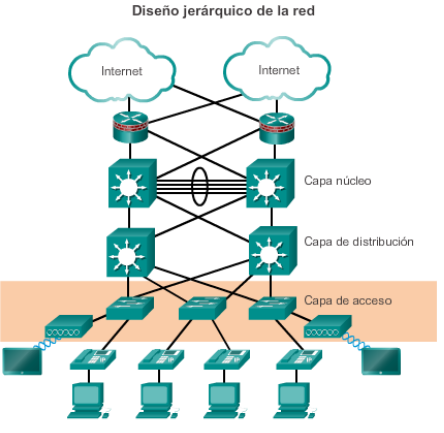
\includegraphics[scale=0.60]{jerarquico}
\end{center}

\subsubsection{ Modelo de n\'ucleo colapsado}
\begin{definicion}[]
{
 combina la capa de distribuci\'on y la capa n\'ucleo
 }
\end{definicion}
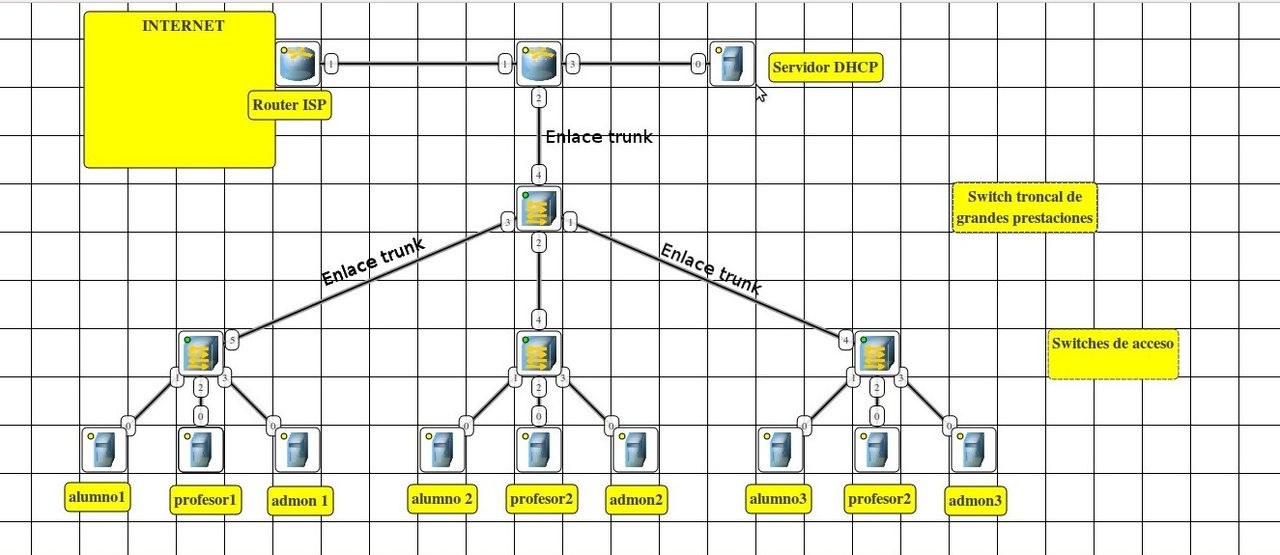
\includegraphics[scale=0.33]{colapsada}

El modelo de dise\~no jer\'arquico es el que implementaremos en el proyecto presente.

\subsection{SEDE AYACUCHO}
\subsubsection{Red central}
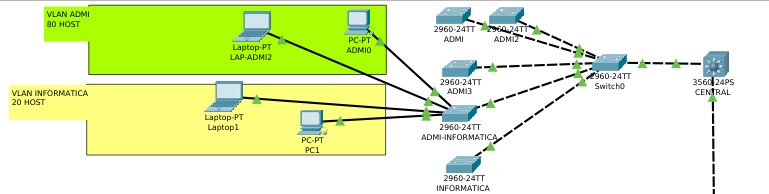
\includegraphics[scale=0.54]{img/central.png} 
\begin{definicion}[]
{
En la red central planteamos dise\~nar un modelo jer\'arquico simple (lo adecuado ser\'ia agregar redundancia en la capa de distribuci\'on). La capa de acceso cuenta con 5 switchs de capa 2(80 host unidad administrativa y 20 unidad inform\'atica). 3 switchs ser\'an propios de vlan admi, 1 ser\'a compartido y 1 ser\'a parcialmente de vlan inform\'atica ya que no alcanza a ocupar todos los puertos disponibles(23 ya que 1 est\'a destinado a conectarse al switch central).El switch central nos permite extender la conectividad ya que con el podemos conectar hasta 23 switches en esta red.
}
\end{definicion}

\subsubsection{Red Campus}
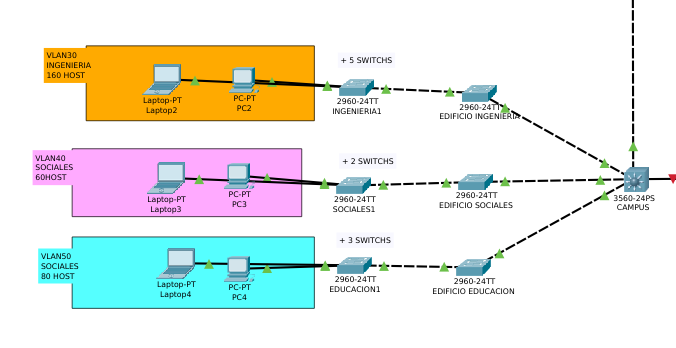
\includegraphics[scale=0.54]{img/CAMPUS.png} 
\begin{definicion}[]
{
En la red del campus se propone hacer una implementaci\'on igual a la anterior, para el primer edificio que cuenta con 160 host se har\'a uso de 160 host que son equivalentes a 7 switchs(23*7), sobrando inclusive 1 puerto.
\\
Para el edificio de sociales se necesitan 60 host para lo cual se hace uso de 3 switchs (3*23), sobrando inclusive 9 puertos.
\\
Para el edificio de educacion que requiere de 80 host se hace uso de 4 switchs (4*23) sobrando inclusive 12 puertos.
}
\end{definicion}




\subsection{SEDE LIMA}
\subsubsection{Red cono sur}
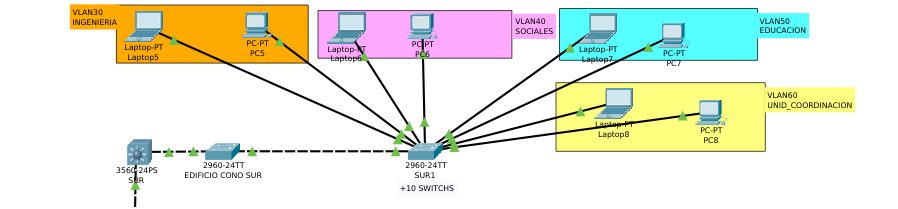
\includegraphics[scale=0.48]{img/CONOSUR.png} 
\begin{definicion}[]
{
Se requiere 240 host por ello, se hace uso de 11 swits (11*23), sobrando 13 puertos.
}
\end{definicion}


\subsubsection{Red cono centro}
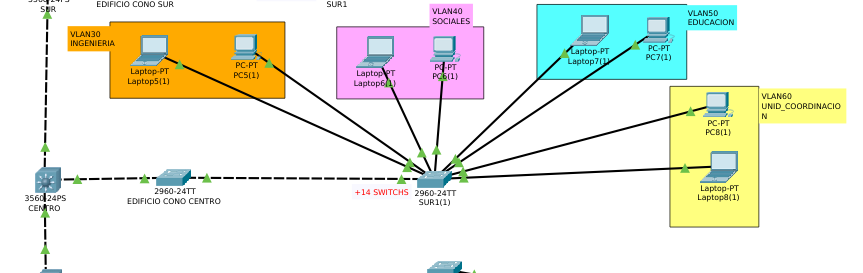
\includegraphics[scale=0.48]{img/CONOCENTRO.png} 
\begin{definicion}[]
{
Se requiere 340 host por ello, se hace uso de 15 swits (15*23), sobrando 5 puertos.
}
\end{definicion}


\subsubsection{Red cono norte}
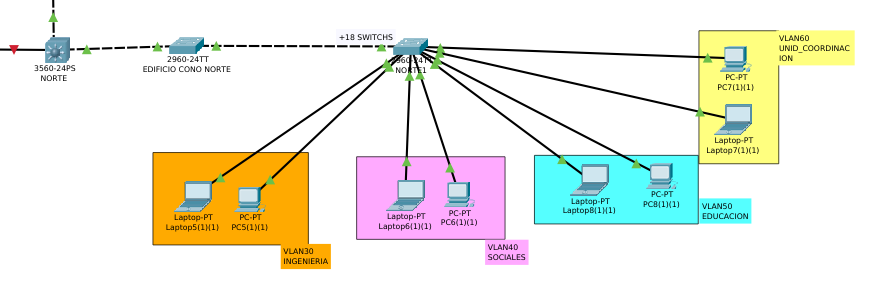
\includegraphics[scale=0.48]{img/CONONORTE.png} 
\begin{definicion}[]
{
Se requiere 420 host por ello, se hace uso de 19 swits (19*23), sobrando 17 puertos.
}
\end{definicion}



\subsection{SEDE HUANCAYO}
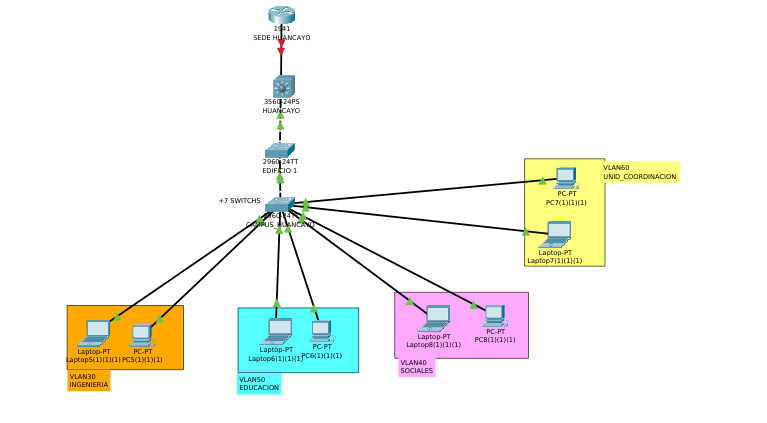
\includegraphics[scale=0.6]{img/HUANCAYO.png} 

\begin{definicion}[]
{
Se requiere 180 host por ello, se hace uso de 8 swits (8*23), sobrando 4 puertos.
}
\end{definicion}

\subsection{SEDE AREQUIPA}
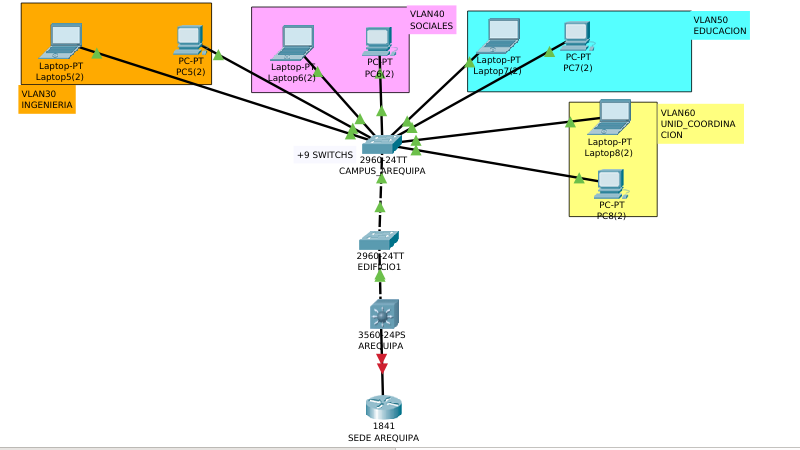
\includegraphics[scale=0.6]{img/AREQUIPA.png} 

\begin{definicion}[]
{
Se requiere 220 host por ello, se hace uso de 10 swits (10*23), sobrando 10 puertos.
}
\end{definicion}


\section{Tipo de direcci\'on IP p\'ublica}
\begin{caja}[]
{
La direcci\'on IP puede ser p\'ublica o privada: La direcci\'on IP p\'ublica es un n\'umero \'unico que identifica nuestra red desde el exterior. La direcci\'on IP privada  identifica a un dispositivo conectado en nuestra red interna.
}
\end{caja}
 Haremos uso de dos tipos de direcciones:
\begin{definicion}[]
{
Direcci\'on externa:
	Direcci\'on externa para la comunicaci\'on de sedes esta direcci\'on es conocida y servir\'a como seguridad para la salida de cada sede. Cada router permitir\'a convertir la direcci\'on interna a la externa al comunicarse a otra sede.
 \\
 Nuestra direcci\'on externa ser\'a 179.6.194.12 que es de tipo B y es la que contratamos.
 }
\end{definicion}
\begin{definicion}[]
{
Direcci\'on Interna:
	Esta direcci\'on es la que segmentaremos para cada sede y esta ser\'a una direcci\'on interna.
 \\
 Nuestra direcci\'on externa ser\'a 172.16.0.0 que es de tipo B.
 }
\end{definicion}


\section{estructura de conexi\'on para la interconexi\'on entre routers}
Se har\'a una conexi\'on NAT con sobrecarga para poder brindar seguridad a la comunicaci\'on entre sedes.\\
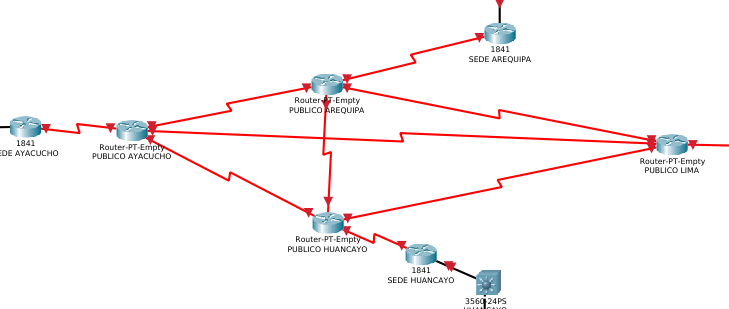
\includegraphics[scale=0.55]{img/ROUTERNAT.png} 

\section{segmentaci\'on de subredes IP}

\subsection{Sede Central Ayacucho}
Usaremos la ip INTERNA: 172.16.0.0
\\
Para hallar usaremos el m\'etodo de VLSM, con el tercer y cuarto octeto. \\

\\
Entonces tenemos:

IP: 172.16.0.0
\\
\textbf{ORDENAMOS LOS HOST QUE SE REQUIERE DE CADA SUCURSAL:}
\\

\begin{definicion}[]
{
\begin{enumerate}[label=\itembolasazules{}]
\item Sede cono-norte: 420 computadoras
\item Sede cono-centro: 340 computadoras
\item Sede campus-ayacucho: 300 computadoras
\item Sede cono-sur: 240 computadoras
\item Sede Arequipa: 220 computadoras
\item Sede Huancayo: 180 computadoras
\item Sede central-ayacucho: 100 computadoras\\
\end{enumerate}
}
\end{definicion}

\newpage
%\usepackage{pdflscape}%poner en vertical hoja en el index
\begin{landscape}
\textheight = 15cm
\textwidth = 25cm % Ancho
\topmargin = -2cm
\oddsidemargin = -1cm
Para poder hacer la segmentaci\'on necesitamos: \\
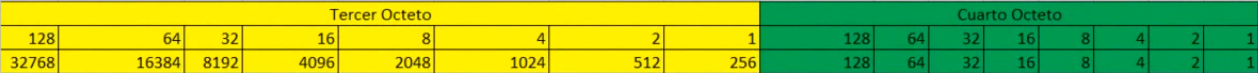
\includegraphics[scale=0.5]{img/octetos.png}
\\
sabemos que la primera subred es la que nos dan por defecto entonces: \\



% Please add the following required packages to your document preamble:
% \usepackage[table,xcdraw]{xcolor}
% If you use beamer only pass "xcolor=table" option, i.e. \documentclass[xcolor=table]{beamer}
\begin{table}[htbp]
\begin{tabular}{|l|l|l|l|l|l|l|}
\hline
\rowcolor[HTML]{32CB00} 
\textbf{subred}  & Host & \textbf{dir sub red} & \textbf{rango ip} & \textbf{broadcast} & \textbf{mascara} & \textbf{/MSR} \\ \hline
cono-norte       & 420  & 172.16.0.0           &                   &                    &                  &               \\ \hline
cono-centro      & 340  &                      &                   &                    &                  &               \\ \hline
campus-ayacucho  & 300  &                      &                   &                    &                  &               \\ \hline
cono-sur         & 240  &                      &                   &                    &                  &               \\ \hline
Arequipa         & 220  &                      &                   &                    &                  &               \\ \hline
Huancayo         & 180  &                      &                   &                    &                  &               \\ \hline
central-Ayacucho & 100  &                      &                   &                    &                  &               \\ \hline
\end{tabular}
\end{table}


Para hallar la siguiente sub red: vemos que requiere 420 host buscamos este numero en la tabla o un valor mayor.
\\
En este caso para 420 es 512; por lo tanto n= 2\\
Quiere decir que la siguiente sub red tendr\'a un salto de 2, asi tenemos:



% Please add the following required packages to your document preamble:
% \usepackage[table,xcdraw]{xcolor}
% If you use beamer only pass "xcolor=table" option, i.e. \documentclass[xcolor=table]{beamer}
\begin{table}[htbp]
\begin{tabular}{|l|l|l|l|l|l|l|}
\hline
\rowcolor[HTML]{32CB00} 
\textbf{subred}  & Host & \textbf{dir sub red} & \textbf{rango ip} & \textbf{broadcast} & \textbf{mascara} & \textbf{/MSR} \\ \hline
cono-norte       & 420  & 172.16.0.0           &                   &                    &                  &               \\ \hline
cono-centro      & 340  & 172.16.2.0           &                   &                    &                  &               \\ \hline
campus-ayacucho  & 300  &                      &                   &                    &                  &               \\ \hline
cono-sur         & 240  &                      &                   &                    &                  &               \\ \hline
Arequipa         & 220  &                      &                   &                    &                  &               \\ \hline
Huancayo         & 180  &                      &                   &                    &                  &               \\ \hline
central-Ayacucho & 100  &                      &                   &                    &                  &               \\ \hline
\end{tabular}
\end{table}


realizamos el mismo paso para los dem\'as:\\
y nos quedaria:


% Please add the following required packages to your document preamble:
% \usepackage[table,xcdraw]{xcolor}
% If you use beamer only pass "xcolor=table" option, i.e. \documentclass[xcolor=table]{beamer}
\begin{table}[htbp]
\begin{tabular}{|l|l|l|l|l|l|l|}
\hline
\rowcolor[HTML]{32CB00} 
\textbf{subred}  & Host & \textbf{dir sub red} & \textbf{rango ip} & \textbf{broadcast} & \textbf{mascara} & \textbf{/MSR} \\ \hline
cono-norte       & 420  & 172.16.0.0           &                   &                    &                  &               \\ \hline
cono-centro      & 340  & 172.16.2.0           &                   &                    &                  &               \\ \hline
campus-ayacucho  & 300  & 172.16.4.0           &                   &                    &                  &               \\ \hline
cono-sur         & 240  & 172.16.6.0           &                   &                    &                  &               \\ \hline
Arequipa         & 220  & 172.16.7.0           &                   &                    &                  &               \\ \hline
Huancayo         & 180  & 172.16.8.0           &                   &                    &                  &               \\ \hline
central-Ayacucho & 100  & 172.16.9.0           &                   &                    &                  &               \\ \hline
\end{tabular}
\end{table}



Para hallar la mascara de sub red lo que hacemos es sumar todos los n\'umeros que esten a la derecha de n incluido n; es decir para la sub red 135.40.0.0 n=2
entonces sumamos: \\
128+64+32+16+8+4+2 = 254\\
Entonces la MSR seria = 255.255.254.0\\
repetimos para todas las sub redes:
% Please add the following required packages to your document preamble:
% \usepackage[table,xcdraw]{xcolor}
% If you use beamer only pass "xcolor=table" option, i.e. \documentclass[xcolor=table]{beamer}
\begin{table}[htbp]
\begin{tabular}{|l|l|l|l|l|l|l|}
\hline
\rowcolor[HTML]{32CB00} 
\textbf{subred}  & Host & \textbf{dir sub red} & \textbf{rango ip} & \textbf{broadcast} & \textbf{mascara} & \textbf{/MSR} \\ \hline
cono-norte       & 420  & 172.16.0.0           &                   &                    & 255.255.254.0    & /23           \\ \hline
cono-centro      & 340  & 172.16.2.0           &                   &                    & 255.255.254.0    & /23           \\ \hline
campus-ayacucho  & 300  & 172.16.4.0           &                   &                    & 255.255.254.0    & /23           \\ \hline
cono-sur         & 240  & 172.16.6.0           &                   &                    & 255.255.255.0    & /24           \\ \hline
Arequipa         & 220  & 172.16.7.0           &                   &                    & 255.255.255.0    & /24           \\ \hline
Huancayo         & 180  & 172.16.8.0           &                   &                    & 255.255.255.0    & /24           \\ \hline
central-Ayacucho & 100  & 172.16.9.0           &                   &                    &                  &               \\ \hline
\end{tabular}
\end{table}

En el caso de la central de ayacucho vemos que se pasa al 4 octeto en ese caso lo que hacemos es buscar ahi un numero >= a 100 entonces n=128 y los que estan a la derecha en el cuarto octeto no seria nadie; por ello quedaria 128\\
Entonces el MSR seria 255.255.255.128\\

% Please add the following required packages to your document preamble:
% \usepackage[table,xcdraw]{xcolor}
% If you use beamer only pass "xcolor=table" option, i.e. \documentclass[xcolor=table]{beamer}
\begin{table}[htbp]
\begin{tabular}{|l|l|l|l|l|l|l|}
\hline
\rowcolor[HTML]{32CB00} 
\textbf{subred}  & Host & \textbf{dir sub red} & \textbf{rango ip} & \textbf{broadcast} & \textbf{mascara} & \textbf{/MSR} \\ \hline
cono-norte       & 420  & 172.16.0.0           &                   &                    & 255.255.254.0    & /23           \\ \hline
cono-centro      & 340  & 172.16.2.0           &                   &                    & 255.255.254.0    & /23           \\ \hline
campus-ayacucho  & 300  & 172.16.4.0           &                   &                    & 255.255.254.0    & /23           \\ \hline
cono-sur         & 240  & 172.16.6.0           &                   &                    & 255.255.255.0    & /24           \\ \hline
Arequipa         & 220  & 172.16.7.0           &                   &                    & 255.255.255.0    & /24           \\ \hline
Huancayo         & 180  & 172.16.8.0           &                   &                    & 255.255.255.0    & /24           \\ \hline
central-Ayacucho & 100  & 172.16.9.0           &                   &                    & 255.255.255.128  & /25           \\ \hline
\end{tabular}
\end{table}


Terminamos de llenar las ips y nos quedaria:

% Please add the following required packages to your document preamble:
% \usepackage[table,xcdraw]{xcolor}
% If you use beamer only pass "xcolor=table" option, i.e. \documentclass[xcolor=table]{beamer}
\begin{table}[htbp]
\begin{tabular}{|l|l|l|l|l|l|l|l|l|}
\hline
\rowcolor[HTML]{32CB00} 
\textbf{subred}  & \textbf{Host} & \textbf{dir sub red} & \textbf{gateway} & \textbf{primer ip} & \textbf{ultimo ip} & \textbf{broadcast} & \textbf{mascara} & \textbf{/MSR} \\ \hline
cono-norte       & 420           & 172.16.0.0           & 172.16.0.1       & 172.16.0.2         & 172.16.1.254       & 172.16.1.255       & 255.255.254.0    & /23           \\ \hline
cono-centro      & 340           & 172.16.2.0           & 172.16.2.1       & 172.16.2.2         & 172.16.3.254       & 172.16.3.255       & 255.255.254.0    & /23           \\ \hline
campus-ayacucho  & 300           & 172.16.4.0           & 172.16.4.1       & 172.16.4.2         & 172.16.5.254       & 172.16.5.255       & 255.255.254.0    & /23           \\ \hline
cono-sur         & 240           & 172.16.6.0           & 172.16.6.1       & 172.16.6.2         & 172.16.6.254       & 172.16.6.255       & 255.255.255.0    & /24           \\ \hline
Arequipa         & 220           & 172.16.7.0           & 172.16.7.1       & 172.16.7.2         & 172.16.7.254       & 172.16.7.255       & 255.255.255.0    & /24           \\ \hline
Huancayo         & 180           & 172.16.8.0           & 172.16.8.1       & 172.16.8.2         & 172.16.8.254       & 172.16.8.255       & 255.255.255.0    & /24           \\ \hline
central-Ayacucho & 100           & 172.16.9.0           & 172.16.9.1       & 172.16.9.2         & 172.16.9.126       & 172.16.9.127       & 255.255.255.128  & /25           \\ \hline
\end{tabular}
\end{table}


\end{landscape}


\section{segmentaci\'on de subredes VLAN}

Realizaremos la segmentaci\'on por puertos.\\
\subsection{Ayacucho}

\subsubsection{sede central administrativa}
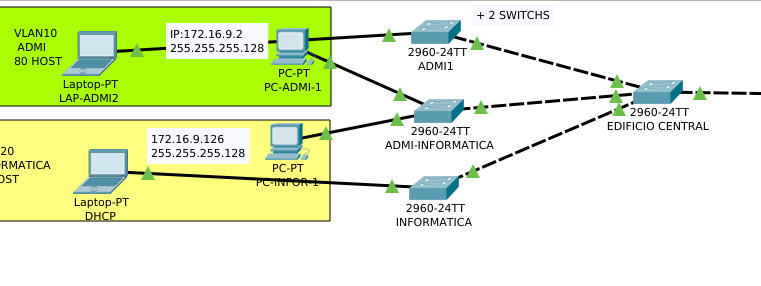
\includegraphics[scale=0.52]{img/vlancentral.png} 

\textbf{CONFIGURAMOS LOS SWITCHS}
 
 \subsubsection{Campus Universitario}
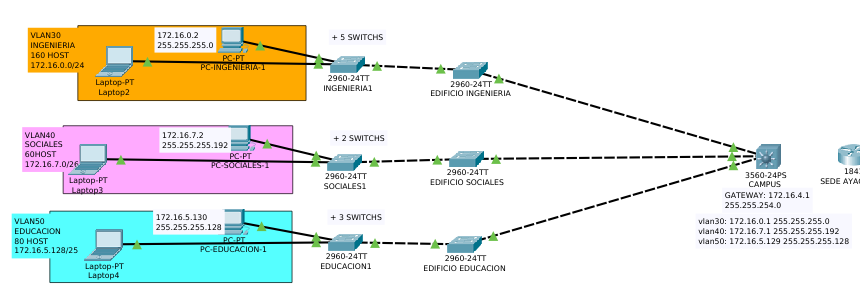
\includegraphics[scale=0.35]{img/VLANCAMPUS.png} 
\subsection{Conexi\'on sucursal Lima}
\subsubsection{sucursal cono norte}
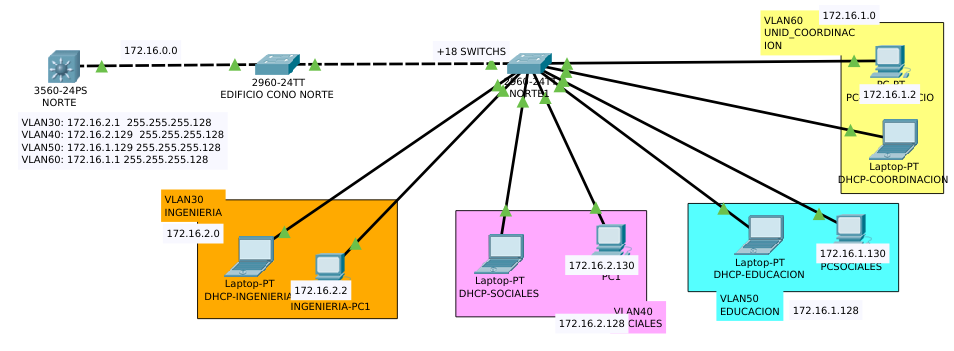
\includegraphics[scale=0.45]{img/VLANNORTE.png} \\
\subsubsection{sucursal cono centro}
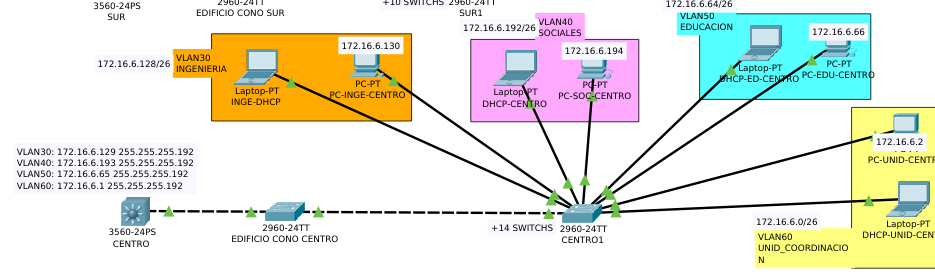
\includegraphics[scale=0.45]{img/VLANCENTRO.png} 

\subsubsection{sucursal cono sur}
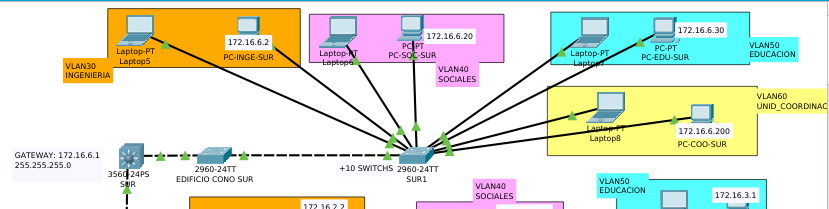
\includegraphics[scale=0.45]{img/VLANSUR.png} 

\subsection{Conexi\'on sucursal Arequipa}
ser\'an de igual manera que de la sucursal de lima.
\\
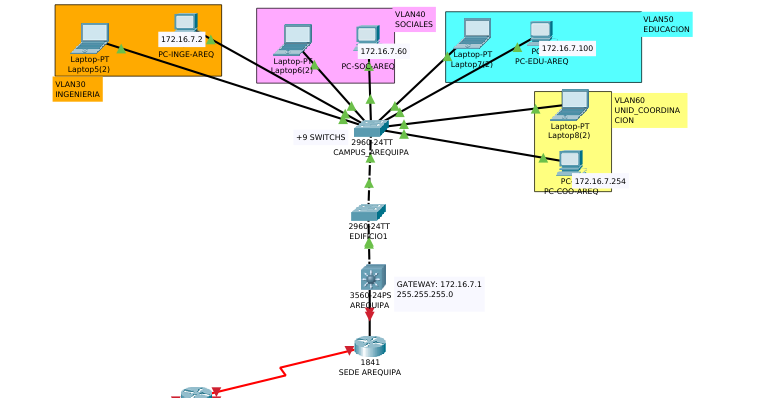
\includegraphics[scale=0.45]{img/VLANAREQUIPA.png} 

\subsection{Conexi\'on sucursal Huancayo}
ser\'an de igual manera que de la sucursal de lima.
\\
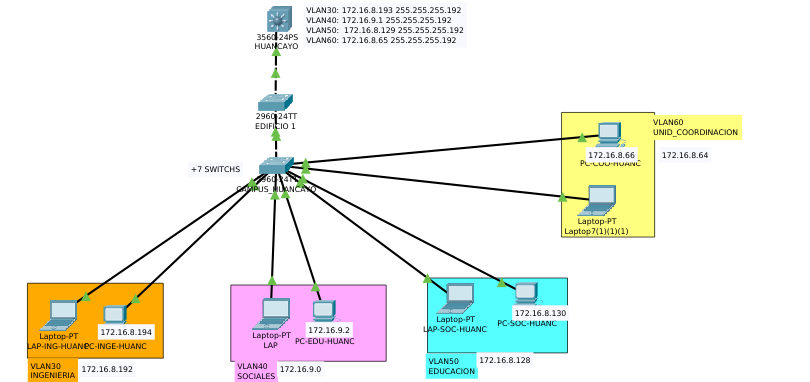
\includegraphics[scale=0.45]{img/VLANHUANCAYO.png} 


\section{\¿Le parece acertada la decisi\'on del Jefe de Inform\'atica?, Sustente en profundidad su respuesta para cada caso}
\subsection{SEGMENTACI\'ON DE REDES}
\begin{definicion}[]
{
\begin{enumerate}[label=\itembolasazules{}]
\item Qu\'e se adquiera una direcci\'on IP p\'ublica y que se utilice
segmentaci\'on basada en subredes IP para cada una de las sucursales.
\item Qu\'e cada una de las Facultades sean segmentadas utilizando VLAN.
\end{enumerate}
}
\end{definicion}
Para este caso la utilizaci\'on de una ip publica mejora mucho la seguridad de una red ya que al salir hacia una wan o internet estamos propensos a sufrir suplantacion de identidad entre muchas otras cosas.
\\
la ip publica hace que esto sea mas dificil de realizar ya q siempre saldremos al exterior con una ip publica de conocimiento de todos.\\

NO solo las facultades deben de ser segmentadas en Vlans sino todas las unidades involucradas para poder tener asi un mejor control en la red.
\subsection{LOCALIZACI\'ON DE SERVIDORES}
\begin{definicion}[]
{
\begin{enumerate}[label=\itembolasazules{}]
\item Que la Oficina de Inform\'atica en Ayacucho tenga.

\begin{enumerate}[label=\itembolas{}]
\item 01 Servidor de DHCP, que asigne direcciones IP din\'amicas a las
sedes de Ayacucho, Arequipa y Huancayo.
\item 1 Servidor de DNS.
\item 1 Servidor Web que contenga las p\'aginas web de cada una de las
sedes (Ayacucho, Lima, Arequipa y Huancayo).
\end{enumerate}

\item Qu\'e la Sede Lima Cono Central tenga: 01 Servidor para servicio de DHCP, que asigne direcciones IP
din\'amicas a las tres sedes de Lima solamente.
\end{enumerate}
}

\end{definicion}
Lo mas recomendable deber\'ia ser tener todos esos servidores en un ambiente m\'as adecuado, ya que no se menciona que la casona cuente con lo requerido para que se cumplan los est\'andares basicos que se requiere.
\\
Se deberia de separar con una granja de servidores y asi provea servicio a todos; los servidores deber\'ian de estar ubicados todos juntos en un lugar adecuado.


%=========FIN objetivos=========

\end{document}
